\chapter{Implementation \label{chap:implementation}}



\epigraph{Python is the "most powerful language you can still read".}{\textit{Paul Dubois \\ Lead developer for Numerical Python and Pyfort }}

This chapter familiarises the reader with the creation of a curve follow project in RoboDK. Firstly, it focuses on the specifics of programming FANUC robotic arms. Secondly, it gives a short introduction to setting up a curve follow project in RoboDK. Subsequently, it describes the RoboDK API, and in the end, it deals with the problematics of post processors and the modification of post processors.

\section{FANUC robotic arms programming specifics}

\subsection{FANUC Roboguide}

FANUC Roboguide is a proprietary robotic arm simulation and offline programming tool developed by the FANUC corporation. FANUC Roboguide is in many ways similar to RoboDK.  Like RoboDK, it supports the creation of robotic arm stations, importing of CAD files and CAD--to--path features. The main difference is that Roboguide is limited to FANUC robotic arms and FANUC related technologies and procedures. In contrast, RoboDK is not limited to one robotic arm manufacturer and is universal and expandable. FANUC Roboguide is used in this study to compile the created robotic arm controller programs and upload them to the robotic arm controller. FANUC Roboguide offers several simulation software options tailored for specific robotic arm applications:

\begin{itemize}

\item FANUC Roboguide HandlingPRO -- simulating material handling applications including loading/unloading, packaging, assembly and material removal,
\item FANUC Roboguide PaintPRO -- simulating painting applications,
\item FANUC Roboguide WeldPRO -- simulating robotic arc welding processes,
\item FANUC Roboguide PalletPRO and PalletTool -- simulating palletizing applications.

\end{itemize}

An example of a FANUC Roboguide station is shown in Figure \ref{fig:roboguide}. The version of FANUC Roboguide used in this study is 8.30104.00.35 (Rev. K) \cite{roboguide}. 

\begin{figure}[h]
    \centering
    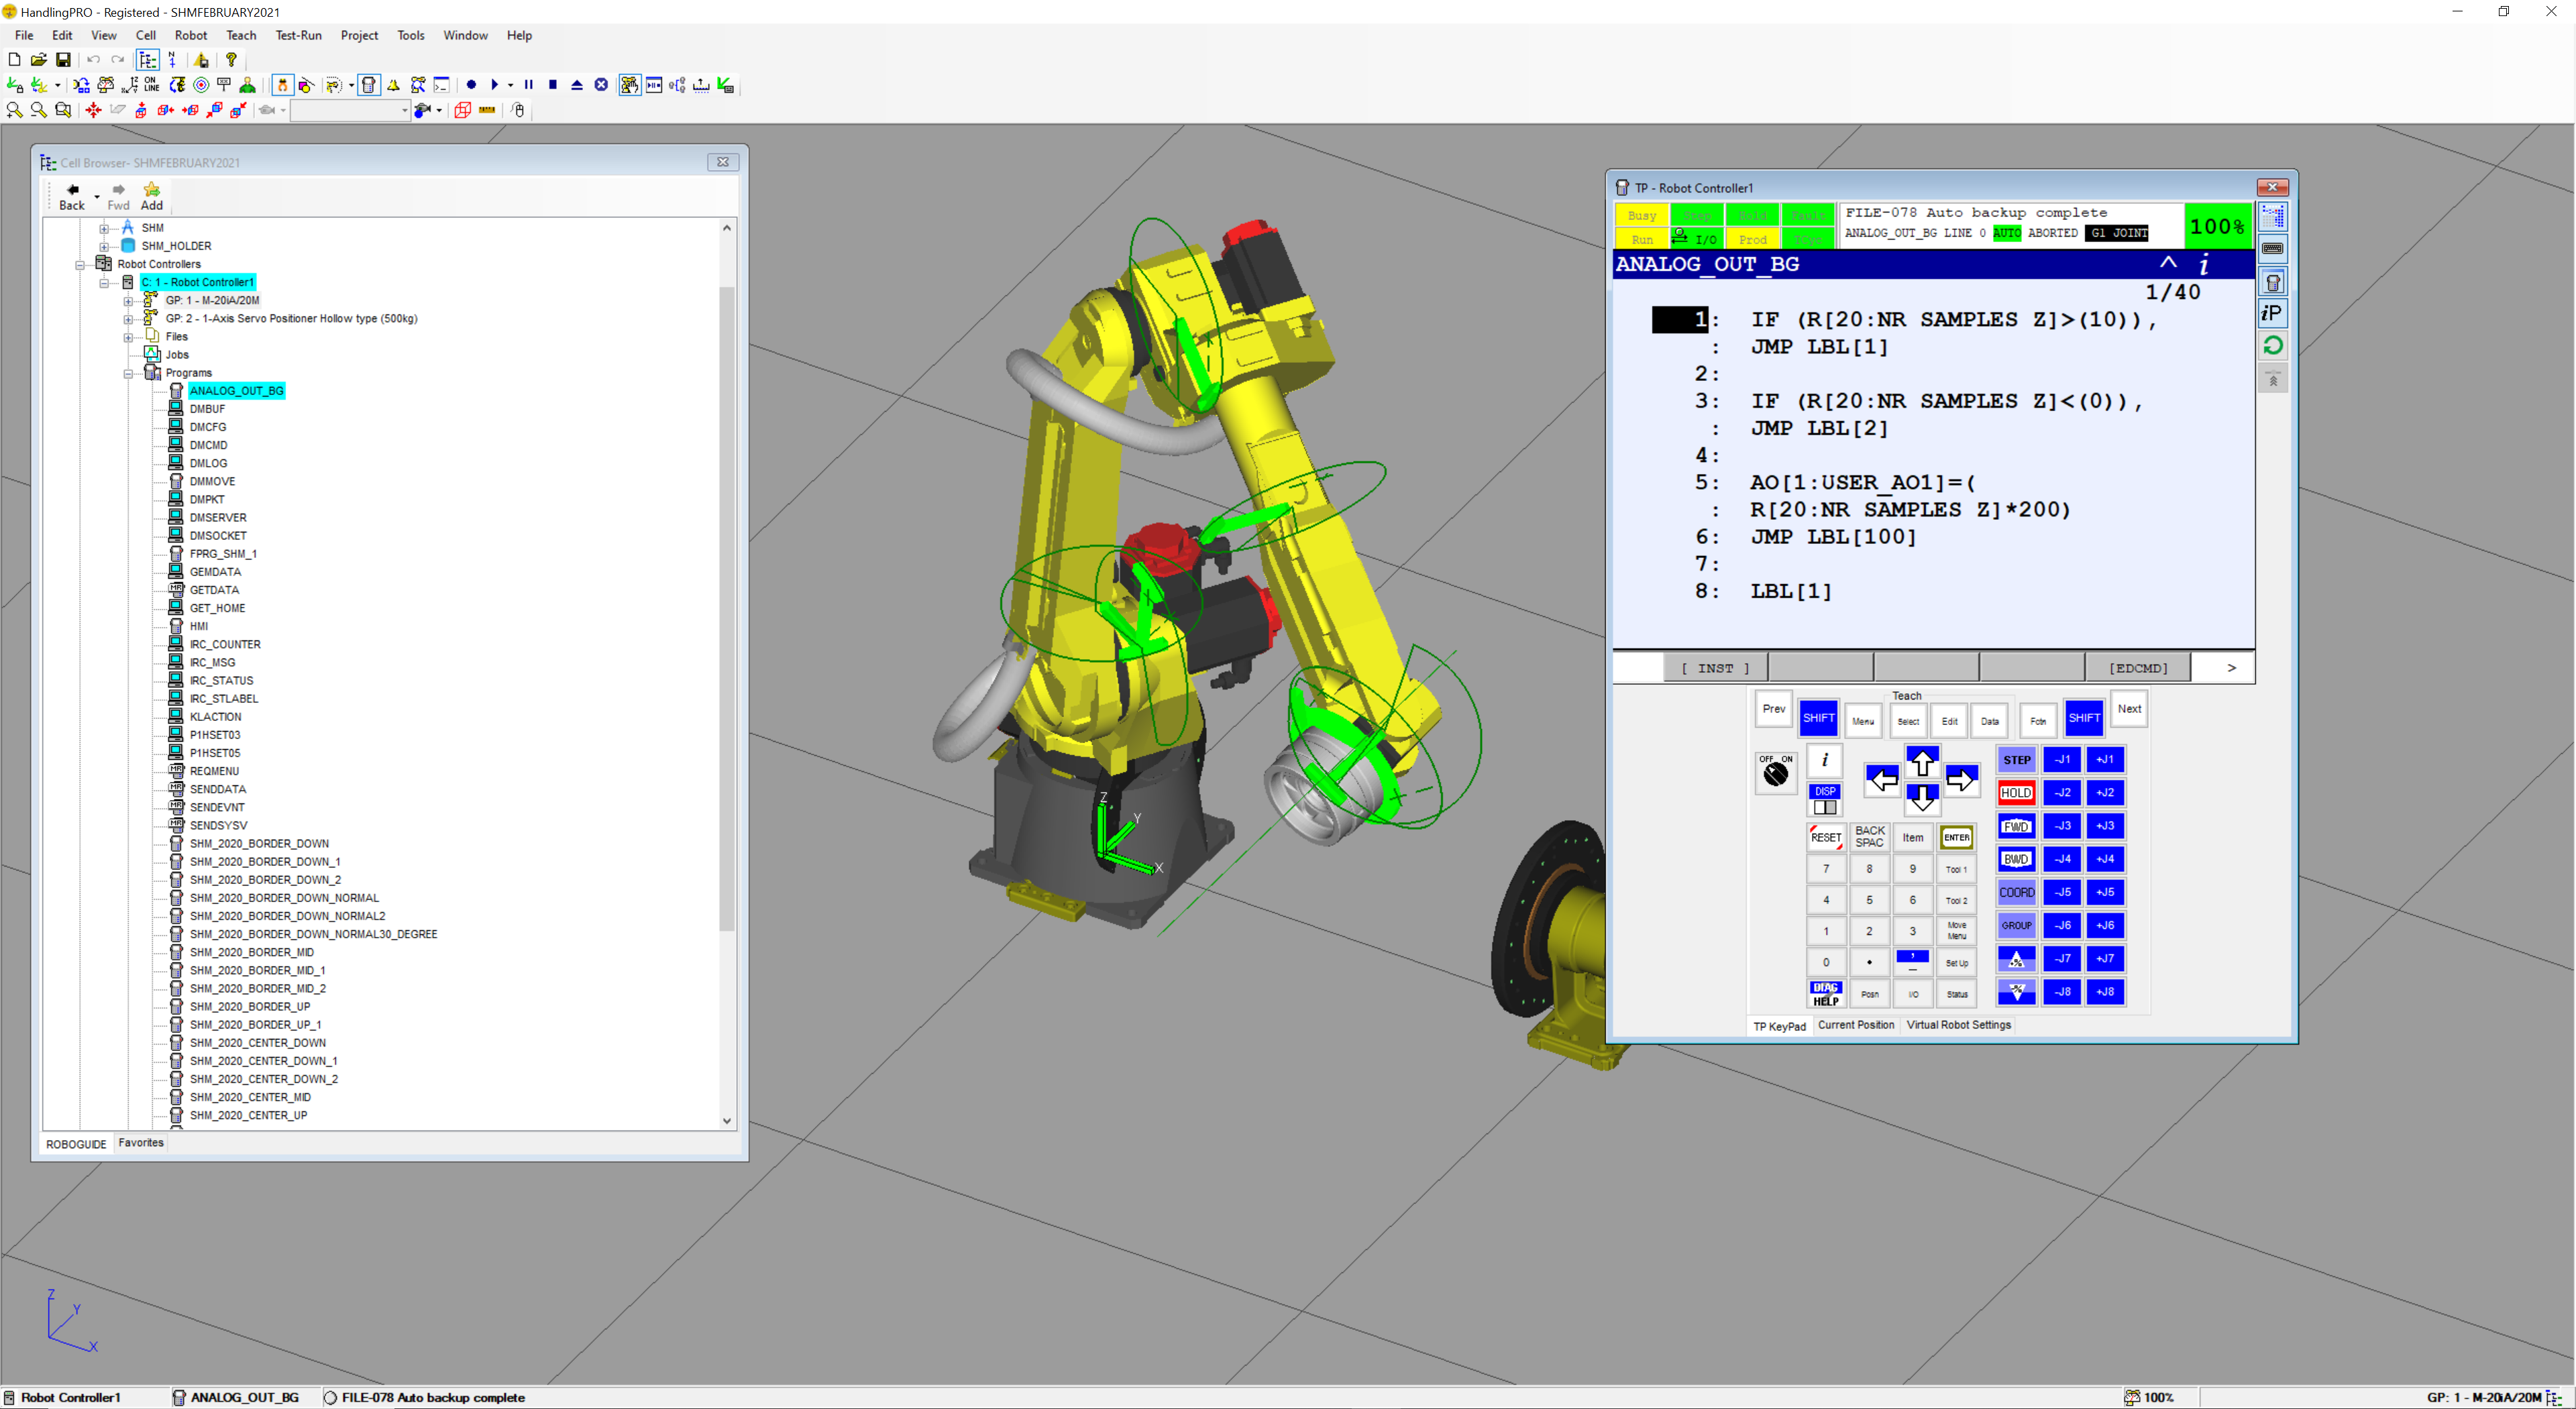
\includegraphics[width=0.9\linewidth]{img/roboguide.PNG}
    \caption{FANUC Roboguide workcell -- user interface example}
    \label{fig:roboguide}
\end{figure}

\subsection{FANUC robotic arm controller programming languages}

The FANUC company implements two programming languages for programming their robotic arm controllers: teach pendant (TP) or KAREL. The TP language is mainly used for motion control of the robotic arm and the programs are usually edited via the pendant. TP programs are either binary files (\inline{.tp} file extension) or can be human--readable ASCII files (\inline{.ls} file extension). The syntax of the TP language is described in great detail in the \emph{SYSTEM R-30iB and R-30iB MATE HandlingTool Setup and Operations Manual} \cite{fanuchandling}. The KAREL language is a high--level language and does not support robotic arm movement instructions. KAREL is mainly used to implement program logic. KAREL programs can not be edited using a pendant. The syntax of the KAREL language is covered in the \emph{FANUC Robotics SYSTEM R-30iA Controller KAREL Reference Manual} \cite{karelmanual}.



\subsection{Teach pendant program structure}

A program element is a segment of a program. A TP program is a collection of program elements with the purpose of executing an application.  Figure \ref{fig:tp} shows an example of a TP program with some typical program elements. A TP program is typically composed of the following program elements:

\begin{itemize}

\item program header information -- includes information such as program name, comment, group mask, program type, application mask, write protection setting, and cycle time, 
\item UTOOL and FRAME number entries -- specify the frame and tool used,
\item line numbers -- assigned to each program instruction,
\item motion instructions -- include commands that tell the robotic arm where and how to move,
\item program instructions for logic, I/O, data handling, program control, advanced functions,
\item remarks -- annotate the program,
\item program end marker -- indicates that there are no more instructions in the program.

\end{itemize}

\begin{figure}[h]
    \centering
    
\includegraphics[width=0.9\linewidth]{img/tp.jpg}
    \caption[Example of a TP program with some typical program elements]{Example of a TP program with some typical program elements \protect\cite{fanuchandling} }
    \label{fig:tp}
\end{figure}

A motion instruction is the most important type of program element. A motion instruction directs the robot to move in a specified way to a specific location in the workcell using a specified speed. Figure \ref{fig:motion} shows a typical example of a motion instruction. A motion instruction consists of:

\begin{itemize}

\item motion type -- how the robot moves to the position,
\item position indicator symbol -- indicates that the robot is at the taught position,
\item positional information -- where the robot moves,
\item termination type -- how the robot ends the move to the position,
\item speed -- how fast the robot moves to a position,
\item motion options -- additional commands that perform specific tasks during robot motion.

\end{itemize}

\begin{figure}[h]
    \centering
    
\includegraphics[width=0.9\linewidth]{img/motion_command.jpg}
    \caption[Example of motion instruction]{Example of motion instruction \protect\cite{fanuchandling}}
    \label{fig:motion}
\end{figure}

\begin{comment}



\subsection{FANUC robotic arm controller programming languages}

The FANUC company implements two programming languages for programming their robotic arm controllers: teach pendant (TP) or KAREL. The TP language is mainly used for motion control of the robotic arm and the programs are usually edited via the pendant. TP programs are either binary files (\inline{.tp} file extension) or can be human--readable ASCII files (\inline{.ls} file extension). The syntax of the TP language is described in great detail in the \emph{SYSTEM R-30iB and R-30iB MATE HandlingTool Setup and Operations Manual} \cite{fanuchandling}. The KAREL language is a high--level language and does not support robotic arm movement instructions. KAREL is mainly used to implement program logic. KAREL programs can not be edited using a Teach pendant. The syntax of the KAREL language is covered in the \emph{FANUC Robotics SYSTEM R-30iA Controller KAREL Reference Manual} \cite{karelmanual}.

\subsection{Compiling a FANUC TP program}

Only a TP program in binary format can be run on FANUC robotic arm controllers. Because RoboDK creates TP programs as human--readable ASCII files, the TP programs need to be converted to binary format before uploading them to the robotic arm controller. Two options to convert \inline{.ls} programs to \inline{.tp} programs exist:

\begin{enumerate}
\item the ASCII Upload option must be loaded on the robotic arm controller. After uploading an \inline{.ls} file to the controller, it is automatically converted to a \inline{.tp} file,
\item the program is compiled and uploaded either using the WinOLPC  tools via Roboguide or using the WinOLPC tools directly \cite{fanuchandling}. The WinOLPC tools are located in \inline{C:/Program File(x86)/FANUC/WinOLPC/bin} in the Windows operating system.

\end{enumerate}

\end{comment}


\subsection{Compiling a FANUC teach pendant program}

Only a TP program in binary format can be run on FANUC robotic arm controllers. Because RoboDK creates TP programs as human--readable ASCII files, the TP programs need to be converted to binary format before uploading them to the robotic arm controller. Two options to convert \inline{.ls} programs to \inline{.tp} programs exist:

\begin{enumerate}
\item the ASCII Upload option must be loaded on the robotic arm controller. After uploading an \inline{.ls} file to the controller, it is automatically converted to a \inline{.tp} file,
\item the program is compiled and uploaded either using the WinOLPC  tools via Roboguide or using the WinOLPC tools directly \cite{fanuchandling}. The WinOLPC tools are located in \inline{C:/Program File(x86)/FANUC/WinOLPC/bin} in the Windows operating system.

\end{enumerate}

\section{Robot machining projects in RoboDK}

The applications of robot machining in industry are numerous. Some applications include:

\begin{itemize}

    \item milling,
    \item drilling,
    \item chamfering,
    \item deburring.

\end{itemize}

RoboDK supports three types of robot machining projects:

\begin{itemize}

    \item robot machining projects -- a robotic arm path is created from an Numerical Control (NC) file,
    \item curve follow projects -- robotic arm follows a curve path in 3D space, 
    \item point follow projects -- robotic arm follows a path defined by points in 3D space.

\end{itemize}

The process of setting up a curve follow project in RoboDK is described in the following sections. In laser shock peening, the laser (representing the tool) is static, and the robot holds the object. Therefore, a curve follow project with a constant tool orientation is set up in RoboDK \cite{machiningproject}.

\subsection{Setting up a curve follow project in RoboDK}
\label{sec:setting_up}

A curve follow project in RoboDK must at least consist of one robot, one tool, and one reference frame. The situation described is a so--called remote TCP situation, i.e., the Tool Center Point (TCP) is fixed in the station, and the robot holds the object. The TCP in our project is represented by the laser beam. 
The user has to execute the following steps to set up a basic curve follow project and to generate a vendor--specific robot program: 

\begin{enumerate}

\item create and import the robotic arm path to RoboDK using preferred CAD software,

\item mount the robot path as a tool in RoboDK,

\item create reference frame (optionally import CAD of manufactured part) in RoboDK station, 

\item create curve follow project: \inline{Utilities} $\rightarrow$ \inline{Curve follow project},

\item open the curve follow project settings. A window similar to the one displayed in Figure \ref{fig:curvefollow} will open, 

\item modify curve follow project settings:

    \begin{itemize}

        \item \inline{Robot}: the robotic arm holding the object,
        \item \inline{Reference}: the frame representing the remote TCP,
        \item \inline{Tool}: the robotic arm path.
        
    \end{itemize}
    
\item change \inline{Select algorithm} option to: \inline{Robot holds object & follows path},

\item select \inline{Update project}. RoboDK automatically generates a preprocessed robot program for the actual station,

\item right--click the preprocessed program, select post processor and generate program. The \inline{.ls} program for the actual station will be opened in the default RoboDK text editor,

\item compile the program and export the program to the FANUC robot controller using FANUC Roboguide or WinOLPC tools \cite{curvefollow}.
    
\end{enumerate}

\begin{figure}[h]
    \centering
    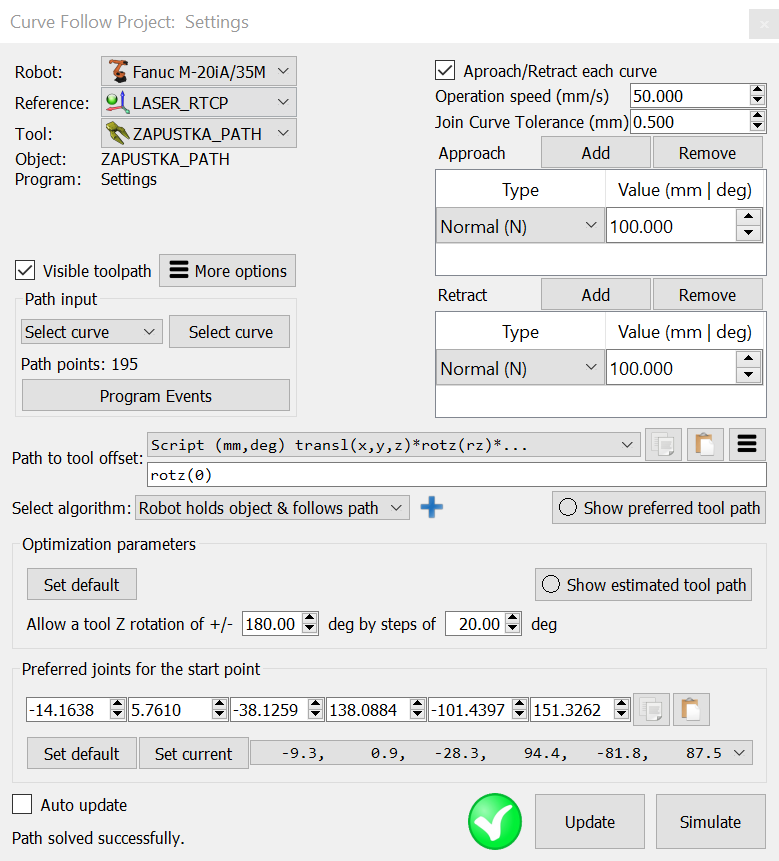
\includegraphics[width=0.9\linewidth]{img/curve_follow_settings.PNG}
    \caption{Curve follow project settings in RoboDK}
    \label{fig:curvefollow}
\end{figure}

\section{RoboDK API}

An application interface (API) is a set of features an application provides to the user via a high--level programming language. The RoboDK API dramatically expands the potential of RoboDK. The RoboDK API is implemented in Python, C\#, C++, Visual Basic (.NET) and Matlab.  The Python API is the most extensive and is used in this study. The RoboDK API facilitates the execution of the following tasks:

\begin{itemize}
    
 \item automating simulations -- macro scripts for repetitive tasks such as tool changing, pick and place applications.

 \item offline programming -- using the RoboDK API methods to create programs for specific robotic arm controllers. The pre--processed \inline{.pyc} file created in RoboDK's GUI is executed directly by the post processor. The post processor defines the rules for vendor--specific robotic arm controller program generation. 

 \item online programming -- using RoboDK API to move robots and retrieve their current position in real time. RoboDK connects to the robotic arm controller using robot drivers.

\end{itemize}

The elegance of this approach is that the same program written in a high--level programming language can be used for all three of the above--mentioned tasks \cite{robodkapi}. 

\subsection{Python API for RoboDK}

Python is an interpreted high--level programming language. The Python API for RoboDK uses Python 3, although most features are compatible with Python 2 also. The RoboDK API for Python consists of the following modules:

\begin{itemize}
    \item \inline{robolink} module -- this module represents the link between RoboDK and the high--level programming language,
    \item \inline{item} module -- any item from the RoboDK item tree can be retrieved.  An item can be a robotic arm, a reference frame, a tool, an object, or a specific project,
    \item \inline{robodk} module -- a module with a robotics toolbox for pose operations. All post processors depend on the \inline{robodk} module .
\end{itemize}

The modules are located in the folder  \inline{C:/RoboDK/Python/} in the Windows operating system. This folder is included in the \inline{PYTHONPATH} system variable. The Python API is accompanied with examples. These examples are located in the folders \newline \inline{C:/RoboDK/Library/Scripts} and  \inline{C:/RoboDK/Library/Macros}  in the Windows operating system \cite{robodkapipython}.

\section{RoboDK post processors}

A post processor specifies how robot programs must be generated for a specific robot controller and are used when robot programs are generated offline. Post processors serve as tools to convert the simulation to vendor--specific robot programs. All RoboDK post processors are placed in the \inline{C:/RoboDK/Posts} folder in the Windows operating system. All post processors rely on the \inline{robodk} module. The \inline{robodk} module is a robotics toolbox for Python, based on \href{http://petercorke.com/Robotics_Toolbox.html}{Peter Corke’s Robotics Toolbox} \cite{robodkapipython}. 

\subsection{RoboDK post processor workflow}

The creation of a program that is compatible with a FANUC robotic arm controller consists of three steps. These steps are shown in Figure \ref{workflow}:

\begin{enumerate}
  \item create a program in a curve follow project in RoboDK,   
  \item generate a preprocessed/universal \inline{.pyc} file using RoboDK,
  \item generate a vendor--specific robot \inline{.ls} program using the post processor.
\end{enumerate}


\begin{figure}[h]
    \centering
    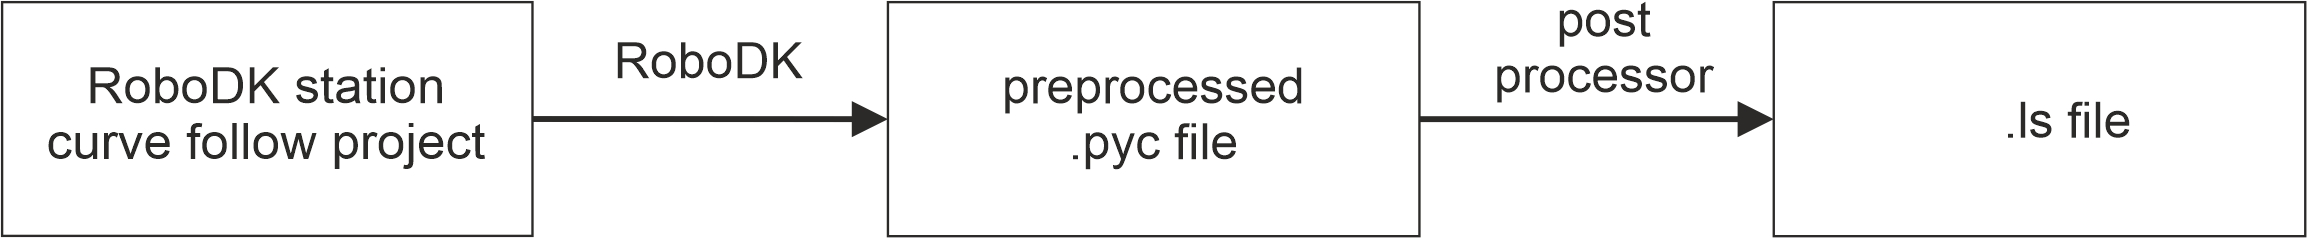
\includegraphics[width=0.9\linewidth]{img/workflow.jpg}
    \caption{RoboDK post processor workflow}
    \label{workflow}
\end{figure}


\subsection{RoboDK preprocessed file}

After creating a program in the curve follow project, but before generating it using a post processor, the program is saved as a preprocessed/universal Python program and saved in a local temporary folder. The post processor defines a \inline{RobotPost} class that generates the desired code. In the Windows operating system, the preprocessed Python files are saved in the user's temporary folder (e.g.: \inline{C:/Users/username/AppData/Temp}). These programs can also be used for debugging new post processors. A code snippet of a preprocessed file is shown in Listing \ref{code:preprocessed_python} \cite{preprocessed}. The three dots (...) denote parts of the code that have been intentionally omitted to keep the source code listing shorter. 




%% this is an example of a minted code with caption and wrapped lines

% this lstlisting form in this example is working perfectly for python 

\begin{lstlisting}[numbers=none,caption={Code snippet of preprocessed program to be executed by post processor},captionpos=b,label={code:preprocessed_python}, language={}]


import sys
import os
sys.path.append(os.path.abspath(r"""C:/RoboDK/Posts/""")) # temporarily add path to POSTS folder

from FANUC_R30iA_decompyle3 import *

def p(x,y,z,r,p,w):
  a = r*math.pi/180.0
  b = p*math.pi/180.0
  c = w*math.pi/180.0
  ca = math.cos(a)
  sa = math.sin(a)
  cb = math.cos(b)
  sb = math.sin(b)
  cc = math.cos(c)
  sc = math.sin(c)
  return Mat([[cb*ca,ca*sc*sb--cc*sa,sc*sa+cc*ca*sb,x], [cb*sa,cc*ca+sc*sb*sa,cc*sb*sa--ca*sc,y], [--sb,cb*sc,cc*cb,z], [0.0,0.0,0.0,1.0]])

print('Total instructions: 140')
r = RobotPost(r"""FANUC_R30iA_decompyle3""",r"""Fanuc M--20iA/35M""",6, axes_type=['R','R','R','R','R','R'], ip_com=r"""127.0.0.1""", api_port=20500, prog_ptr=2172227036784, robot_ptr=2172252511552)

r.ProgStart(r"""Settings""")
r.RunMessage(r"""Program generated by RoboDK v5.2.2 for Fanuc M--20iA/35M on 02/07/2021 17:12:29""",True)
r.RunMessage(r"""Using nominal kinematics.""",True)
r.setZoneData(1.000)
r.setSpeed(1000.000)
r.setFrame(p(1000.3,--445,552.3,0,10.19,--90),--1,r"""LASER_RTCP""")
r.setTool(p(0,0,0,0,0,0),--1,r"""ZAPUSTKA_PATH""")
r.RunMessage(r"""Show ZAPUSTKA_PATH""",True)
r.MoveJ(None,[--9.2878,0.949114,--28.3094,94.4347,--81.8311,87.4811],None)
r.MoveL(p(--14.8303,41.4662,85,105.917,0,180), [--14.8823,2.45519,--28.2667,97.1731,--76.9261,87.0176], [0,0,0])
r.setSpeed(10.000)
r.MoveL(p(0.866853,42.1343,85,94.455,0,180), [--14.6627,3.59506,--28.447,97.1044,--77.1403,75.3963], [0,0,0])

...
...
...

r.setSpeed(1000.000)
r.MoveL(p(--16.1785,41.074,185,107.509,0,180), [--9.29955,0.844572,--28.2678,94.4344,--81.8176,449.114], [0,0,0])
r.ProgFinish(r"""Settings""")
r.ProgSave(r"""C:/Users/marek.boehm/Documents/RoboDK/""", r"""Settings""", False, r"""C:/RoboDK/Other/VSCodium/VSCodium.exe""")


\end{lstlisting}



%% \captionof{listing}{Code snippet of preprocessed program to be executed by post processor}


Let us dive into the source code of this preprocessed file and explain the functionality of some of its methods. The most important method is the \inline{MoveL} function:

%The \inline{p(x,y,z,r,p,w)} method converts the XYZRPW representation to a Pose ($ 4 \times 4 $ matrix).

\begin{comment}
%% RobotPost class
\begin{lstlisting}[frame=lines,numbers=none,breaklines=true]{python}
class samplepost.RobotPost(robotpost=None, robotname=None, robot_axes=6, **kwargs)
\end{lstlisting}

The \inline{RobotPost} class initializes the robot post processor object. 
The parameters of the \inline{RobotPost} class are:

\begin{itemize}

\item \inline{robotpost (string)} -- name of the post processor linked to the preprocessed file,

%% do not highlight anything - then use text
\item \inline{robotname(string)} -- the name of the robotic arm,

\item \inline{robot_axes(string list)} -- type and quantity of robotic arm axes,

\item \inline{**kwargs} -- pass additional arguments to function.

\end{itemize}

All subsequent functions are called upon the \inline{RobotPost} object. The most important method is the \inline{MoveL} function:

\end{comment}
%%%%%%%%%%%%%%%%%%
%% MoveL method
\begin{lstlisting}[frame=lines,numbers=none,breaklines=true]{python}
MoveL(pose, joints, conf_RLF=None)
\end{lstlisting}

The \inline{MoveL} method generates manufacturer-specific code for linear movement. 
The parameters of the \inline{MoveL} method are:

\begin{itemize}

\item \inline{pose (robodk.Mat())} -- pose target of the tool with respect to the reference frame, pose can be \inline{None} if the target is defined as a joint target,

%% do not highlight anything - then use text
\item \inline{joints (float list)} -- robot joints as a list,

\item \inline{conf_RLF (int list)} -- pass additional arguments to function. 

\end{itemize}



%%%%%%%%%%%%%%%%%%
%% ProgStart method
\begin{lstlisting}[frame=lines,numbers=none,breaklines=true]{python}
ProgStart(progname)
\end{lstlisting}

The \inline{ProgStart} method is called when a new program is generated.


The parameters of the \inline{ProgStart} method are:

\begin{itemize}

\item \inline{progname (str)} -- program name.

\end{itemize}

%%%%%%%%%%%%%%%%%%
%% setSpeed method
\begin{lstlisting}[frame=lines,numbers=none,breaklines=true]{python}
setSpeed(speed_mms)
\end{lstlisting}

The \inline{setSpeed} method sets the linear robotic arm speed (in \SI{}{\mm\per\second}).


The parameters of the  \inline{setSpeed} method are:

\begin{itemize}

\item \inline{speed_mms} -- speed in \SI{}{\mm\per\second}.

\end{itemize}

%%%%%%%%%%%%%%%%%%
%% ProgSave method
\begin{lstlisting}[frame=lines,numbers=none,breaklines=true]{python}
ProgSave(folder, progname, ask_user=False, show_result=False)
\end{lstlisting}

The \inline{ProgSave} method saves the program in a format compatible with the corresponding robot controller type. 

The parameters of the \inline{ProgSave} method are:

\begin{itemize}

%% do not highlight anything - then use text
\item \inline{folder (str)} -- folder hint to save the program,

\item \inline{progname (str)} -- program name as a hint to save the program,

\item \inline{ask_user (bool, str)} -- true if the default settings in RoboDK are set to promt the user to select the folder, 

\item \inline{show_result (bool, str)} -- false if the default settings in RoboDK are set to not show the program once it has been saved. Otherwise, a string is provided with the path of the preferred text editor.

\end{itemize}

%%%%%%%%%%%%%%%%%%
%% ProgFinish method
\begin{lstlisting}[frame=lines,numbers=none,breaklines=true]{python}
ProgFinish(progname)
\end{lstlisting}
The \inline{ProgFinish} method is triggered after all the instructions of the program and defines the end of the program.


The parameters of the \inline{ProgFinish} method are:

\begin{itemize}

\item \inline{progname (str)} -- program name.

\end{itemize}

%%%%%%%%%%%%%%%%%%
%%% end of all methods

 Every post processor should implement a set of basic methods to generate programs for robotic arm controllers correctly \cite{postmethods}.


\subsection{Selecting a post processor}

Each robotic arm has a post processor assigned to it by default. The following steps have to be taken to change the post processor of a robotic arm:


\begin{enumerate}
    \item opening the robot panel,
    \item selecting \inline{Parameters},
    \item selecting post processor from drop--down list \cite{selectpost}.
\end{enumerate}

\subsection{Post processor example and post processor example output}

An example of an output of the unmodified R--30iA post processor is shown in Listing \ref{code:unmodified_post}.


\begin{lstlisting}[numbers=none,caption={Code snippet of unmodified R--30iA post processor output},captionpos=b,label={code:unmodified_post}, language={}]
/PROG  Diecast15
/ATTR
OWNER		= MNEDITOR;
COMMENT		= "RoboDK sequence";
PROG_SIZE	= 0;
CREATE		= DATE 31-12-14  TIME 12:00:00;
MODIFIED	= DATE 31-12-14  TIME 12:00:00;
FILE_NAME	= Diecast15;
VERSION		= 0;
LINE_COUNT	= 462;
MEMORY_SIZE	= 0;
PROTECT		= READ_WRITE;
TCD:  STACK_SIZE	= 0,
      TASK_PRIORITY	= 50,
      TIME_SLICE	= 0,
      BUSY_LAMP_OFF	= 0,
      ABORT_REQUEST	= 0,
      PAUSE_REQUEST	= 0;
DEFAULT_GROUP	= 1,*,*,*,*,*,*;
CONTROL_CODE	= 00000000 00000000;
/MN
   1:  ! Program generated by ;
   2:  !  RoboDK v5.2.2 for F ;
   3:  ! anuc M-20iA/35M on 0 ;
   4:  ! 9/08/2021 16:07:49 ;
   5:  ! Using nominal kinema ;
   6:  ! tics. ;
   7:  PR[9,1]=1000.300 ;
   8:  PR[9,2]=-445.000 ;
   9:  PR[9,3]=552.300 ;
  10:  PR[9,4]=-90.000 ;
  11:  PR[9,5]=10.190 ;
  12:  PR[9,6]=0.000 ;
  13:  UFRAME[9]=PR[9] ;
  14:  UFRAME_NUM=9 ;
  15:  PR[9,1]=0.000 ;
  16:  PR[9,2]=0.000 ;
  17:  PR[9,3]=0.000 ;
  18:  PR[9,4]=0.000 ;
  19:  PR[9,5]=0.000 ;
  20:  PR[9,6]=0.000 ;
  21:  UTOOL[9]=PR[9] ;
  22:  UTOOL_NUM=9 ;
  23:  ! Show Diecast15 ;
  24:J P[1] 1% CNT0 ;
  25:L P[2] 50mm/sec CNT0 ;
  26:L P[3] 10mm/sec CNT0 ;
  27:L P[4] 10mm/sec CNT0 ;

...
...
...

461:L P[438] 10mm/sec CNT0 ;
 462:L P[439] 50mm/sec CNT0 ;
/POS
P[1]{
   GP1:
    UF : 9, UT : 9,    
	J1=    -11.825 deg,	J2=    0.745 deg,	J3=    -13.905 deg,
	J4=    69.881 deg,	J5=    -63.946 deg,	J6=    28.200 deg
};
P[2]{
   GP1:
    UF : 9, UT : 9,        CONFIG : 'N U T, 0, 0, 0',
	X =     1.632  mm,	Y =   -67.788  mm,	Z =    73.203  mm,
	W =  -165.352 deg,	P =   -21.879 deg,	R =    21.809 deg
};
P[3]{
   GP1:
    UF : 9, UT : 9,        CONFIG : 'N U T, 0, 0, 0',
	X =     2.074  mm,	Y =   -68.202  mm,	Z =    73.760  mm,
	W =  -165.468 deg,	P =   -21.989 deg,	R =    21.644 deg
};
P[4]{
   GP1:
    UF : 9, UT : 9,        CONFIG : 'N U T, 0, 0, 0',
	X =     2.535  mm,	Y =   -68.640  mm,	Z =    74.302  mm,
	W =  -165.566 deg,	P =   -22.104 deg,	R =    21.494 deg
};

...
...
...

P[439]{
   GP1:
    UF : 9, UT : 9,        CONFIG : 'N U T, 0, 0, -1',
	X =    -1.638  mm,	Y =  -138.500  mm,	Z =   143.912  mm,
	W =  -165.328 deg,	P =    21.824 deg,	R =   -21.741 deg
};
/END

\end{lstlisting}
% \captionof{listing}{Code snippet of unmodified R--30iA post processor output}
% \label{code:unmodified_post}


\section{FANUC R--30iA RoboDK post processor}

The FANUC R--30iA post processor is located in the \inline{C:/RoboDK/Posts/vXX folder}. \inline{XX} is a two--digit number and denotes the post processor version. The FANUC R--30iA post processor comes in the form of a \inline{.pyc} file (compiled bytecode) and needs to be decompiled to a \inline{.py} file with the help of a decompiler. The decompiler used in this study is   \href{https://github.com/rocky/python--decompile3}{decompyle3} \cite{decompyle3}. The FANUC R--30iA post processor is compatible with FANUC R--30iB robotic arm controllers.

\subsection{Modifying the FANUC R--30iA post processor methods} 
\label{sec:modifying}

The user can create a new post processor from scratch or modify an existing post processor. A post processor for a specific robotic arm controller is a single \inline{.py} file. All post processors are placed in the \inline{C:/RoboDK/Posts} folder. A new post processor is added to RoboDK by creating a \inline{.py} file or renaming an existing \inline{.py} file in this folder. By deleting a \inline{.py} file in this folder, the post processor is deleted from the list of post processors. 

The experimental setup of the LSP station at the HiLASE centre links the robotic arm controller to the laser sources. The objective of the post processor modification for the Litron LPY ST 7875-10 2HG laser can be expressed as:

% dirtytalk package

\say{\emph{The laser source is operating at a 1 Hz repetition rate. The post processor for the  R--30iA controller will be modified in such a way that when the robotic arm with the sample is in a position, where the LSP process (individual laser impact area) should be placed, the robotic arm controller sends a command to the laser source to fire exactly one laser pulse onto the desired area and then move on to the next position. This is accomplished by controlling the digital inputs (DIs) and digital outputs (DOs) of the robotic arm controller.}} 

The modification involves the \inline{MoveL} method. The unmodified \inline{MoveL} method generates the following code:


\begin{lstlisting}[frame=lines,numbers=none,breaklines=true, language={}]
n: L P[1] 4mm/sec CNT100;
\end{lstlisting}


where:

\begin{itemize}

    \item \inline{n} -- number of program line, 
    \item \inline{L} -- linear movement,
    \item \inline{P[1]} -- designation of point,
    \item \inline{4mm/sec} -- movement speed,
    \item \inline{CNT100} -- zone data.

\end{itemize}

The modified \inline{MoveL} method should output the following robotic arm controller code to meet the requirements of the post processor:


\begin{lstlisting}[frame=lines,numbers=none,breaklines=true, language={}]
n: WAIT DI[1:SYNCHRONIZATION_IN]=OFF;
n+1: WAIT DI[1:SYNCHRONIZATION_IN]=ON;
n+2: L P[1] 4mm/sec CNT100 TB  0.00sec,DO[5]=PULSE,1.0sec;
n+3: WAIT  DO[5:LASER ON] = OFF;
n+4: WAIT  1.00(sec);
\end{lstlisting}


where:

\begin{itemize}

    \item \inline{n} -- number of program line, 
    \item \inline{WAIT CONDITION} -- wait condition, block code execution until condition  is \inline{True},
    \item \inline{WAIT DI[1:SYNCHRONIZATION_IN]=OFF; WAIT DI[1:SYNCHRONIZATION_IN]=ON;} -- detect rising edge of incoming synchronisation signal,
    \item \inline{TB  0.00sec,DO[5]=PULSE,1.0sec} -- execute command at a certain time before reaching the point,
    \item \inline{P[1]} -- designation of point,
    \item \inline{DO[5]=PULSE,1.0sec} -- rectangular pulse at digital output, pulse duration is one second, this command fires the laser,
    \item \inline{WAIT  1.00(sec)} -- block code execution for a certain amount of time.

\end{itemize}

 Listing \ref{code:originalMoveL} contains the original \inline{MoveL} method of the FANUC R--30iA post processor and Listing \ref{code:modifiedMoveL} contains the modified \inline{MoveL} method \cite{postmethods}. 


\begin{lstlisting}[numbers=none,caption={Code snippet of original MoveL method},captionpos=b,label={code:originalMoveL}, language={}]

    def MoveL(self, pose, joints, conf_RLF=None):
        """Add a linear movement"""
        if self.LAST_POSE is not None:
            if pose is not None:
                if distance(pose.Pos(), self.LAST_POSE.Pos()) < 0.001:
                    if pose_angle_between(pose, self.LAST_POSE) < 0.001:
                        return
        self.page_size_control()
        if pose is None:
            target_id = self.add_target_joints(pose, joints)
            move_ins = 'P[%i] %s %s ;' % (target_id, self.SPEED, self.CNT_VALUE)
        else:
            target_id = self.add_target_cartesian(pose, joints, conf_RLF)
            move_ins = 'P[%i] %s %s ;' % (target_id, self.SPEED, self.CNT_VALUE)
        self.addline(move_ins, 'L')
        self.LAST_POSE = pose


\end{lstlisting}
%\captionof{listing}{Code snippet of original MoveL method}
%\label{code:originalMoveL}


\begin{lstlisting}[numbers=none,caption={Code snippet of modified MoveL method},captionpos=b,label={code:modifiedMoveL}, language={}]

    def MoveL(self, pose, joints, conf_RLF=None):
        """Add a linear movement"""
        if self.LAST_POSE is not None:
            if pose is not None:
                if distance(pose.Pos(), self.LAST_POSE.Pos()) < 0.001:
                    if pose_angle_between(pose, self.LAST_POSE) < 0.001:
                        return
        self.page_size_control()
        
        if pose is None:
            target_id = self.add_target_joints(pose, joints)
            syncro_off = 'WAIT DI[1:SYNCHRONIZATION_IN]=OFF;'
            syncro_on = 'WAIT DI[1:SYNCHRONIZATION_IN]=ON;'
            move_ins = 'P[%i] %s %s TB  0.00sec,DO[5]=PULSE,1.0sec;' % (target_id, self.SPEED, self.CNT_VALUE)
            wait_off = 'WAIT  DO[5:LASER ON] = OFF;'
            wait_on = 'WAIT  1.00(sec);'
            
        else:
            target_id = self.add_target_cartesian(pose, joints, conf_RLF)
            syncro_off = 'WAIT DI[1:SYNCHRONIZATION_IN]=OFF;'
            syncro_on = 'WAIT DI[1:SYNCHRONIZATION_IN]=ON;'
            move_ins = 'P[%i] %s %s TB  0.00sec,DO[5]=PULSE,1.0sec;' % (target_id, self.SPEED, self.CNT_VALUE)
            wait_off = 'WAIT  DO[5:LASER ON] = OFF;'
            wait_on = 'WAIT  1.00(sec);'
            
        self.addline(syncro_off, ' ')
        self.addline(syncro_on, ' ')
        self.addline(move_ins, 'L')
        self.addline(wait_off, ' ')
        self.addline(wait_on, ' ')
        self.LAST_POSE = pose


\end{lstlisting}
%\captionof{listing}{Code snippet of modified MoveL method}
%\label{code:modifiedMoveL}


%%%%%%%%%%%

\subsection{Example output of the modified FANUC R--30iA post processor} 
\label{sec:example}

An example of an output of the modified R--30iA post processor is shown in Listing \ref{code:modified_post}.


\begin{lstlisting}[numbers=none,caption={Code snippet of modified R--30iA post processor output},captionpos=b,label={code:modified_post}, language={}]
/PROG  Diecast15
/ATTR
OWNER		= MNEDITOR;
COMMENT		= "RoboDK sequence";
PROG_SIZE	= 0;
CREATE		= DATE 31-12-14  TIME 12:00:00;
MODIFIED	= DATE 31-12-14  TIME 12:00:00;
FILE_NAME	= Diecast15;
VERSION		= 0;
LINE_COUNT	= 2214;
MEMORY_SIZE	= 0;
PROTECT		= READ_WRITE;
TCD:  STACK_SIZE	= 0,
      TASK_PRIORITY	= 50,
      TIME_SLICE	= 0,
      BUSY_LAMP_OFF	= 0,
      ABORT_REQUEST	= 0,
      PAUSE_REQUEST	= 0;
DEFAULT_GROUP	= 1,*,*,*,*,*,*;
CONTROL_CODE	= 00000000 00000000;
/MN
   1:  ! Program generated by ;
   2:  !  RoboDK v5.2.2 for F ;
   3:  ! anuc M-20iA/35M on 1 ;
   4:  ! 8/09/2021 16:36:30 ;
   5:  ! Using nominal kinema ;
   6:  ! tics. ;
   7:  PR[9,1]=1000.300 ;
   8:  PR[9,2]=-445.000 ;
   9:  PR[9,3]=552.300 ;
  10:  PR[9,4]=-90.000 ;
  11:  PR[9,5]=10.190 ;
  12:  PR[9,6]=0.000 ;
  13:  UFRAME[9]=PR[9] ;
  14:  UFRAME_NUM=9 ;
  15:  PR[9,1]=0.000 ;
  16:  PR[9,2]=0.000 ;
  17:  PR[9,3]=0.000 ;
  18:  PR[9,4]=0.000 ;
  19:  PR[9,5]=0.000 ;
  20:  PR[9,6]=0.000 ;
  21:  UTOOL[9]=PR[9] ;
  22:  UTOOL_NUM=9 ;
  23:  ! Show Diecast15 ;
  24:J P[1] 1% CNT0 ;
  25:  WAIT DI[1:SYNCHRONIZATION_IN]=OFF;
  26:  WAIT DI[1:SYNCHRONIZATION_IN]=ON;
  27:L P[2] 50mm/sec CNT0 TB  0.00sec,DO[5]=PULSE,1.0sec;
  28:  WAIT  DO[5:LASER ON] = OFF;
  29:  WAIT  1.00(sec);
  30:  WAIT DI[1:SYNCHRONIZATION_IN]=OFF;
  31:  WAIT DI[1:SYNCHRONIZATION_IN]=ON;
  32:L P[3] 10mm/sec CNT0 TB  0.00sec,DO[5]=PULSE,1.0sec;
  33:  WAIT  DO[5:LASER ON] = OFF;
  34:  WAIT  1.00(sec);

...
...
...

2210:  WAIT DI[1:SYNCHRONIZATION_IN]=OFF;
2211:  WAIT DI[1:SYNCHRONIZATION_IN]=ON;
2212:L P[439] 50mm/sec CNT0 TB  0.00sec,DO[5]=PULSE,1.0sec;
2213:  WAIT  DO[5:LASER ON] = OFF;
2214:  WAIT  1.00(sec);
/POS
P[1]{
   GP1:
    UF : 9, UT : 9,    
	J1=    -11.825 deg,	J2=    0.745 deg,	J3=    -13.905 deg,
	J4=    69.881 deg,	J5=    -63.946 deg,	J6=    28.200 deg
};
P[2]{
   GP1:
    UF : 9, UT : 9,        CONFIG : 'N U T, 0, 0, 0',
	X =     1.632  mm,	Y =   -67.788  mm,	Z =    73.203  mm,
	W =  -165.352 deg,	P =   -21.879 deg,	R =    21.809 deg
};
P[3]{
   GP1:
    UF : 9, UT : 9,        CONFIG : 'N U T, 0, 0, 0',
	X =     2.074  mm,	Y =   -68.202  mm,	Z =    73.760  mm,
	W =  -165.468 deg,	P =   -21.989 deg,	R =    21.644 deg
};

...
...
...

P[439]{
   GP1:
    UF : 9, UT : 9,        CONFIG : 'N U T, 0, 0, -1',
	X =    -1.638  mm,	Y =  -138.500  mm,	Z =   143.912  mm,
	W =  -165.328 deg,	P =    21.824 deg,	R =   -21.741 deg
};
/END

\end{lstlisting}
% \captionof{listing}{Code snippet of modified R--30iA post processor output}
% \label{code:modified_post}






